
% !TeX spellcheck = de_DE
\documentclass{article}

\usepackage[ngerman]{babel}
\usepackage{graphicx}
\usepackage{indentfirst}
\usepackage{hyperref}
\usepackage{geometry}
\usepackage{changepage}
\usepackage{booktabs}
\usepackage{float}
\usepackage{tabulary}
\usepackage{multirow}

\graphicspath{ {./images/} }

\makeatletter
\newcommand{\sectionauthor}[1]{
	{\parindent 0em \large \scshape Autor: #1 \par \nobreak \vspace*{1em}}
	\@afterheading
}
\newcommand{\specification}[3]{
	{\parindent 0.5em \hangindent 3em \hypertarget{spec:#1:#2}{\textbf{/#1#2/}} #3 \par \nobreak \vspace*{0.5em}}
}
\makeatother

\begin{document}

%--Einleitung--------------------------------------------------------------------------------------------------------------------------------------------------------------------------
\section{Einleitung}
\sectionauthor{Jonas Picker}
Hier wird der Entwurf des Bibliotheksmanagementsystems BiBi beschrieben. Das Dokument bezieht sich auf das Lastenheft von Christian Bachmaier und Armin Größlinger und stellt eine technische Vertiefung unseres Pflichtenhefts dar, welches im Folgenden wiederholt referenziert wird.

%--Systemarchitektur---------------------------------------------------------------------------------------------------------------------------------------------------------------
\section{Systemarchitektur}
\sectionauthor{Ivan Charviakou}

\subsection{Design-Patterns: Schichtenunabhängigkeit}

MVC: Als grundlegendes Design-Pattern sorgt MVC dafür, dass die Model-, Präsentations-, und Steuerungskomponente voneinander weitgehend entkoppelt sind. Dabei implementiert das JSF-Framework per Default Großteile der Präsentations- und Steuerungskomponenten, aber überlässt die Modelkomponente komplett dem Entwickler. Für die Präsentationskomponente werden nämlich vordefinierte UI-Komponente vorgesehen, während der eingebaute Faces-Servlet die Steuerungsaufgabe übernimmt. Durch selbst-definierte Tag-Libraries und Facelets lassen sich diese beiden Komponenten auch ggf. vervollständigen. \vspace{0.5em}

CDI: Die im JSF-Framework eingebaute CDI-Funktionalität ermöglicht eine direkte Kommunikation zwischen abhängigen Komponenten, die durch JSF verwaltet werden. Solche Beziehungen werden dann mit entsprechenden Annotationen, wie ‚@inject‘, gekennzeichnet. In der gegebenen Anwendung trägt CDI dadurch wesentlich zur Intraschichtenkommunikation bei. \vspace{0.5em}

DTOs: Ein Datentransferobjekt (DTO) enthält die Daten zu einer bestimmten Entität oder zu einem zusammenhängenden Ausschnitt aus verschiedenen Entitäten. In der gegebenen Anwendung entspricht das einem Medium, Exemplar, Nutzer, usw. Durch Übergabe von solchen Objekten an verschiedenen Modelschichten, können sie die Daten unabhängig voneinander anpassen oder evaluieren. Als Beispiel prüft im Model die Logikschicht das Format eines E-Mails, während die Sicherheitsschicht SQL-Injection-Attacken in der Eingabe ausschließt. \vspace{0.5em}

DAOs und ihre Fassaden: Zu jedem DTO existiert auch ein Datenzugriffsobjekt (DAO), das bei einer Übergabe eines DTOs die enthaltenen Daten speichert bzw. lädt. Damit mehrere Modelschichten diese Prozeduren eigens erweitern können, verwenden die DTOs in der gegebenen Anwendung den Fassade-Muster. Jede betroffene Schicht verwendet zur Erweiterung eines DAOs nämlich die gleiche Schnittstelle und ruft die Schnittstelle der nächsten Schicht auf. Als Beispiel gibt die Logikschicht ein Passwort im Klartext an und übergibt es an eine DAO-Instanz in der Sicherheitsschicht mittels eines DTOs. Diese Schicht berechnet dann aus dem Klartext einen Hash-Wert und leitet diesen Wert an die DAO-Instanz in der Datenzugriffsschicht weiter. \vspace{0.5em}

Event-Listener: Dadurch, dass JSF verschiedene Arten von Listenern bereitstellt, ist eine stärkere Entkopplung von Schichten möglich. Während Action-, Value-Change-, und Phasenlistener hauptsächlich eine Logikschicht ansprechen, kann beispielweise der eingebaute System-Event-Listener für die unabhängige Initialisierung der Modelschichten sorgen.

\subsection{Design-Patterns: Fehlerbehandlung}

Allgemeiner Testmodus: Es wird ein Testmodus eingeführt, der beim Applikationsstart als Parameter angegeben wird. \vspace{0.5em}

Exceptions: Jede Schicht in der gegebenen Anwendung definiert eigene Checked-Exceptions, die ggf. durch die Schichten hochgeworfen werden. Dabei wird eine solche Exception in jeder Zwischenschicht gefangen in eine eigens definierte Exception umgewandelt bis eine Schicht sie behandelt. Im Gegensatz werden Unchecked-Exceptions nicht behandelt und führen zum Absturz der Anwendung. Während für eine Präsentations- und Logikschicht oft eine GUI-Anzeige als geeignete Behandlung gilt, ist es für jede Schichten anders. Falls es beispielsweise durch eine Checked-Exception in der Datenzugriffsschicht festgestellt wird, dass die verwendete Datenbank nicht mehr erreichbar ist, wird stattdessen dynamisch auf lokale Applikationsdaten zugegriffen. Unter den DAOs in der Datenzugriffsschicht wird somit der Strategy-Muster angewendet. \vspace{0.5em}

Logging: Als Logging-Framework wird der im JDK vordefinierte Framework verwendet. Diese Funktionalität ist nur im Testmodus aktiv und es wird zu einer lokalen Log-Datei geschrieben. \vspace{0.5em}

Validatoren: Das JSF-Framework gibt dem Entwickler die Möglichkeit, Daten auf Korrektheit zu prüfen, bevor sie dem Logikschicht bereitgestellt wird. Da aber komplexere semantische Fehler oft einen größeren Kontext und eine komplexere Behandlung benötigen, wird der Einsatz von diesen Validatoren hauptsächlich auf syntaktische Formattierfehler beschränkt.

\subsection{Design-Patterns: Konkrete Features}

Connection-Pool: Unter einem Pool bezeichnet man eine Sammlung an Objekten, die angefragt, zurückgegeben, und wiederverwendet werden. Dies vermeidet insbesondere die Erzeugung von solchen Objekten, was in Bezug auf Datenbankverbindungen als aufwendig gilt. Da es trivialerweise nur einen solchen Container geben sollte, wird ein Pool auch als Singleton verwendet. Für die gegebene Anwendung wird die HikariCP Implementierung einer solchen Connection-Pool genommen. Beim Testmodus wird die Anzahl an Verbindungen auf eins gesetzt. \vspace{0.5em}

Wartungsthread: In der gegebenen Anwendung kann es vorkommen, dass persistierte Daten oder Daten im Cache mit der Zeit ungültig werden. Du solchen Daten gehört beispielsweise die Gültigkeit von einem Passwortrücksetzungslink. Mit einem Wartungsprozess werden solche Inkonsistenzen erkannt und behoben.

\subsection{Modeldiagramm}

\begin{figure}[H]
	\centering
	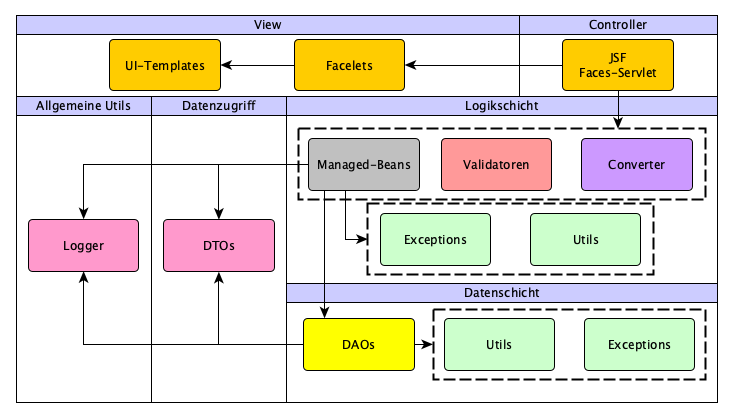
\includegraphics[width = 50em]{Modeldiagramm}
\end{figure}

%--Klassendiagramm---------------------------------------------------------------------------------------------------------------------------------------------------------------

\section{Klassendiagramm}
\sectionauthor{Mohamad Najjar}

%   \begin{landscape}
    \begin{figure}
        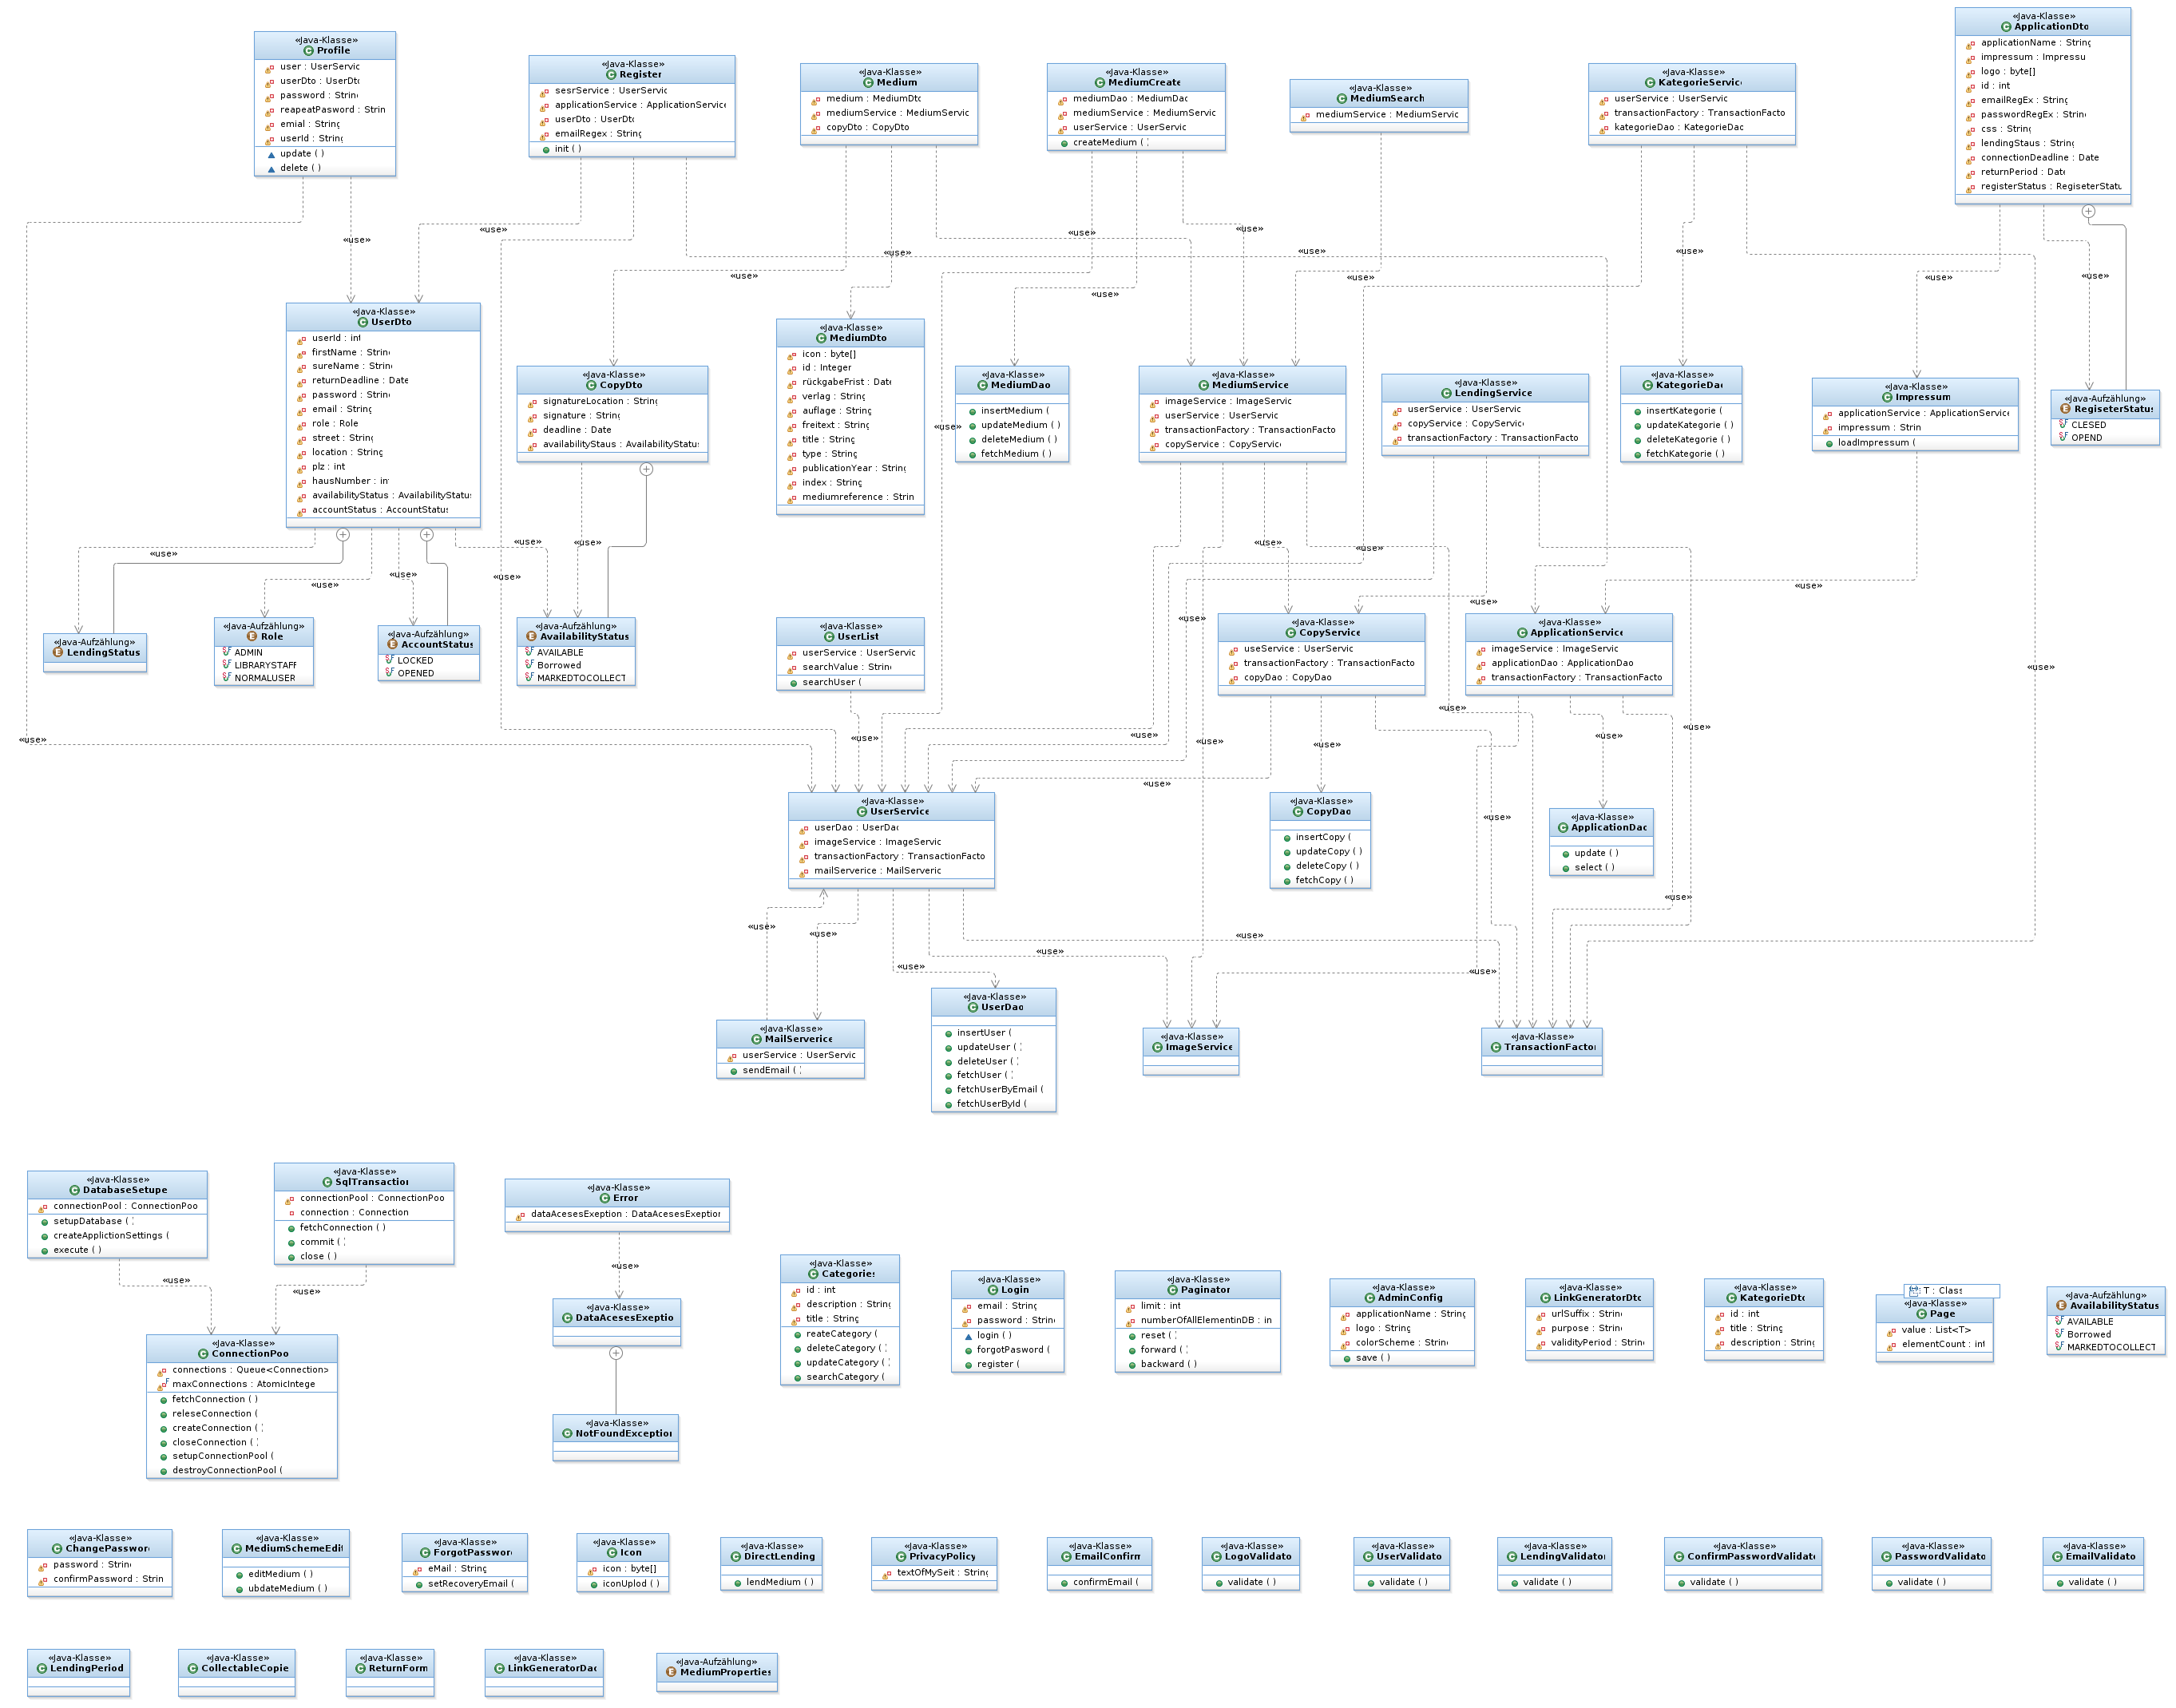
\includegraphics[scale=0.2]{Klassendiagramm.png}
        \caption{Klassendiagramm}
        \label{fig:Klassendiagramm}
    \end{figure}
%    \end{landscape}

%    \begin{landscape}
    \begin{figure}
        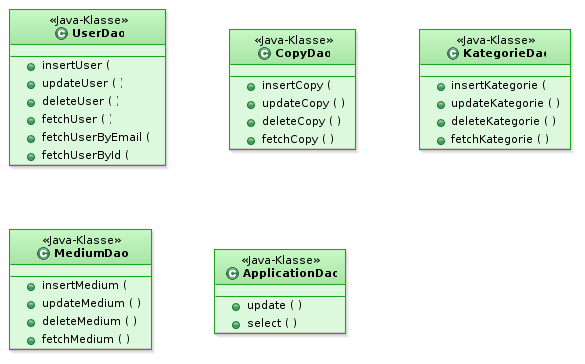
\includegraphics[scale=0.6]{KlassendiagramDao.png}
        \caption{Klassendiagramm der Daos}
        \label{fig:KlassendiagramDao}
    \end{figure}
%    \end{landscape}

%    \begin{landscape}
    \begin{figure}
    \centering
        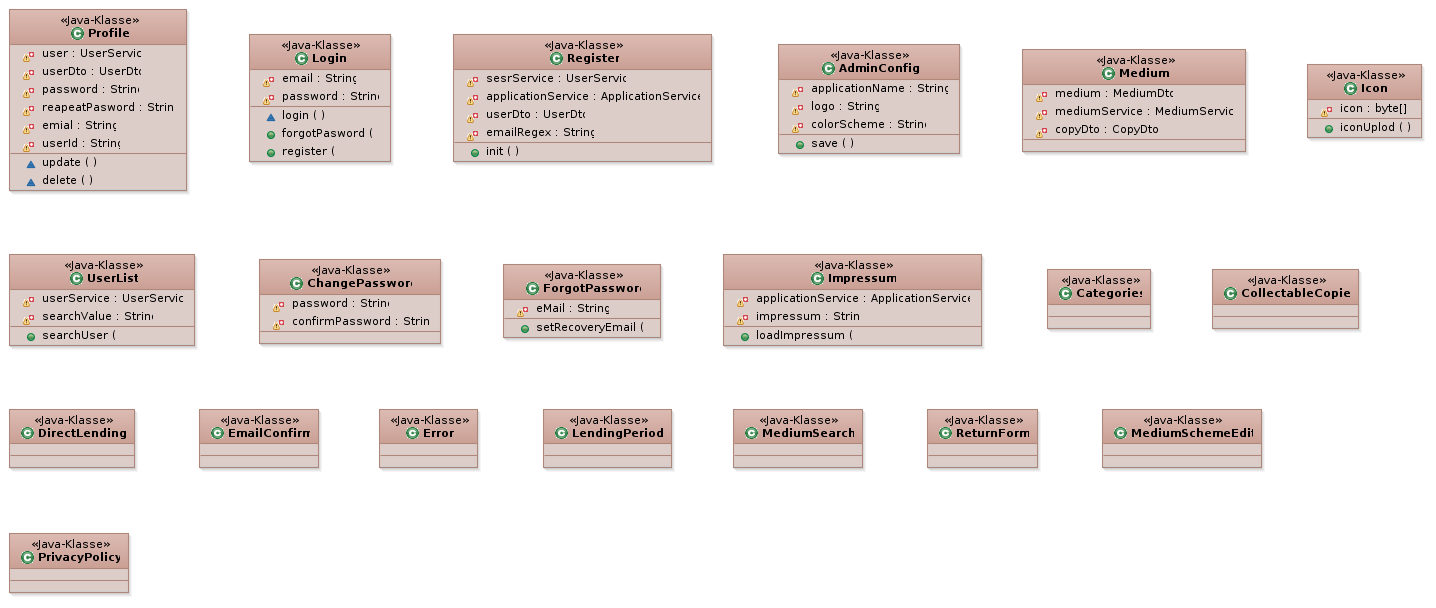
\includegraphics[scale=0.7, angle=270]{KlassendiagramBeans.png}
        \caption{Klassendiagramm der Beans}
        \label{fig:KlassendiagramBeans}
    \end{figure}
%    \end{landscape}

%    \begin{landscape}
    \begin{figure}
        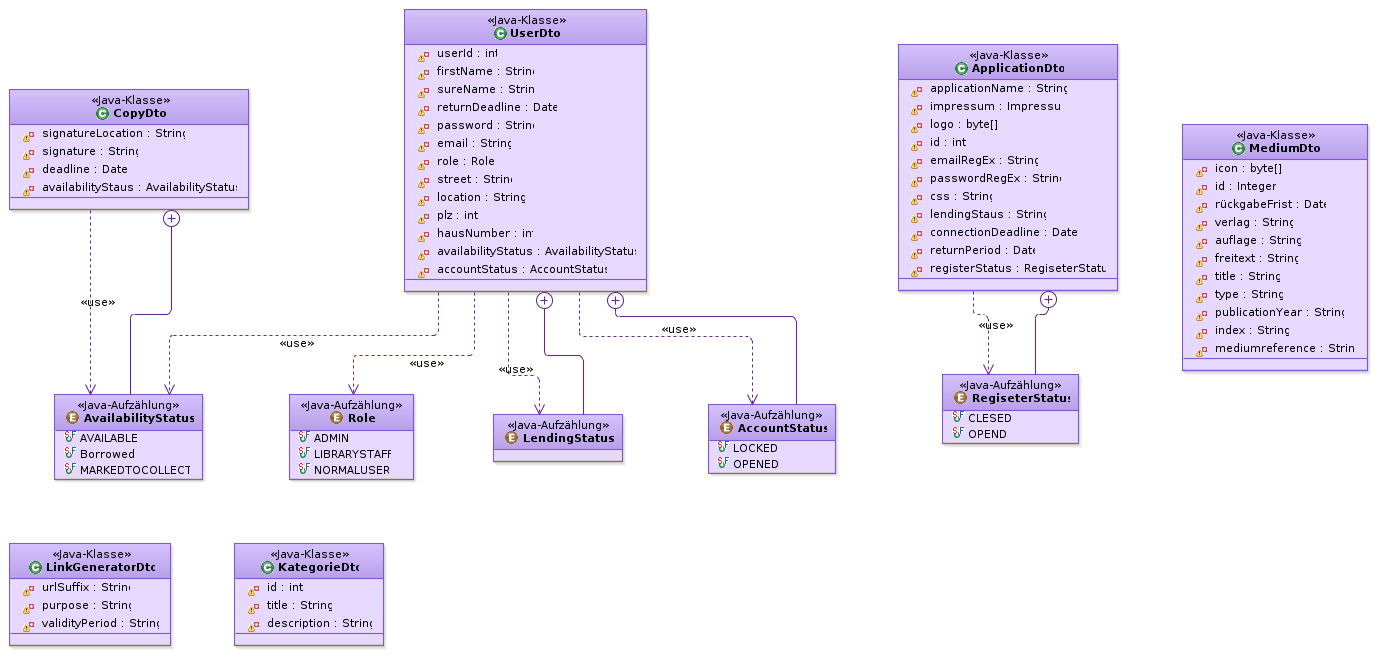
\includegraphics[scale=0.6]{KlassendiagramDtos.png}
        \caption{Klassendiagramm der Dtos}
        \label{fig:KlassendiagrammDto}
    \end{figure}
%    \end{landscape}


%    \begin{landscape}
    \begin{figure}
        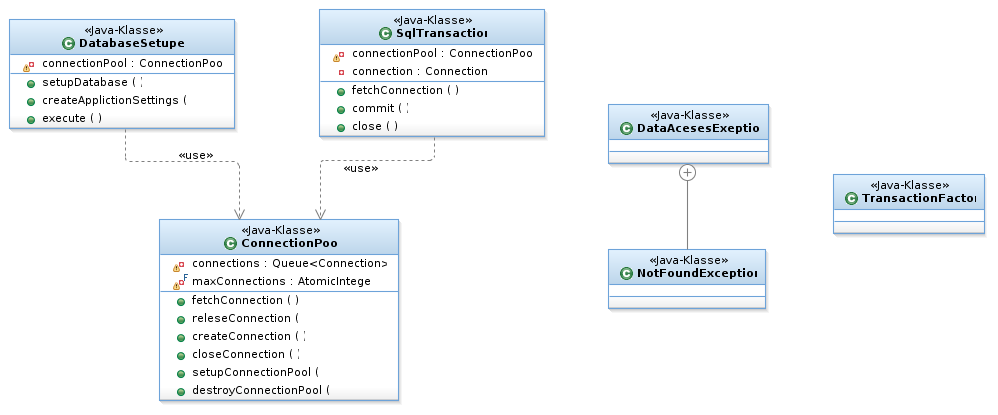
\includegraphics[scale=0.6]{KlassendiagramSystem.png}
        \caption{Klassendiagramm des Systems}
        \label{fig:KlassendiagramSystem}
    \end{figure}
%    \end{landscape}

%    \begin{landscape}
    \begin{figure}
        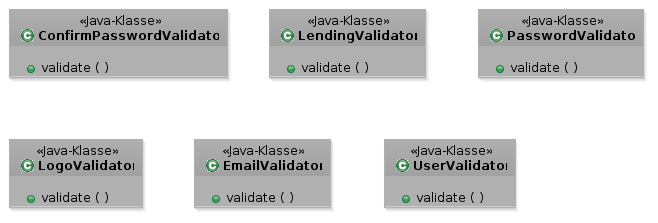
\includegraphics[scale=0.6]{klassendiagramValidator.png}
        \caption{Klassendiagramm des Validator}
        \label{fig:KlassendiagramValidator}
    \end{figure}
%    \end{landscape}


%   \begin{landscape}
    \begin{figure}
        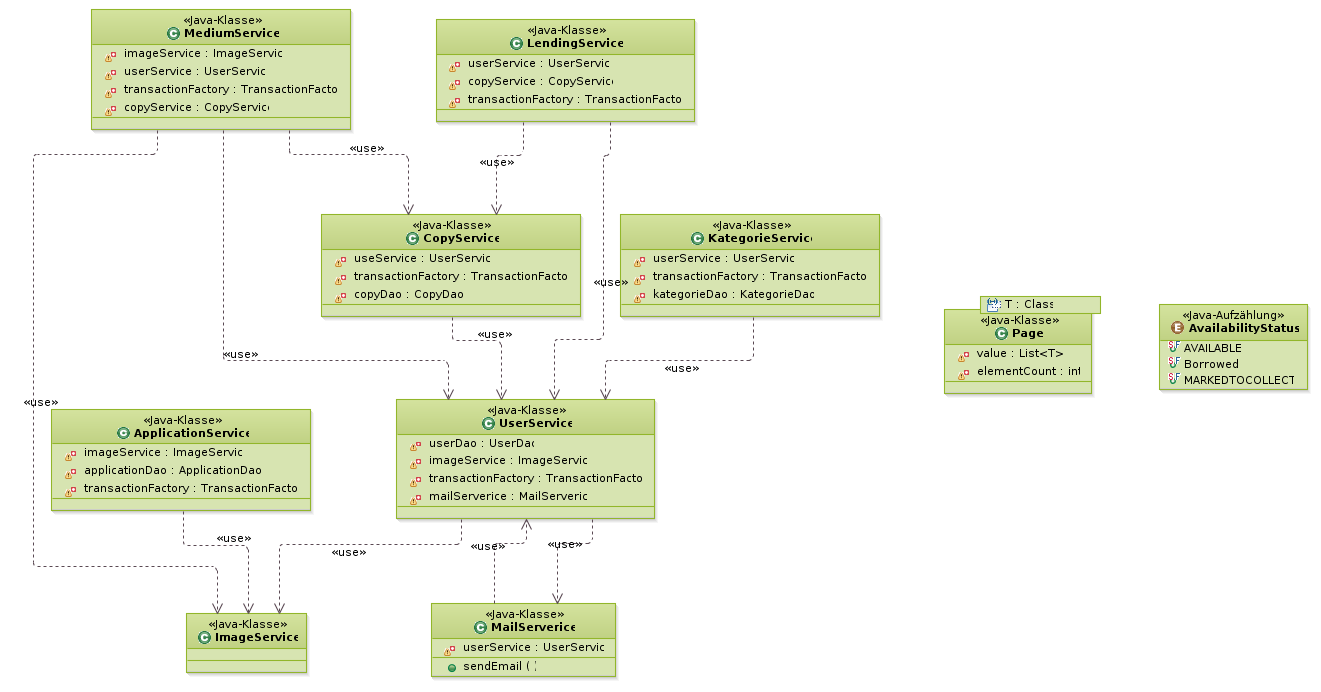
\includegraphics[scale=0.6]{KlassendiagramService.png}
        \caption{Klassendiagramm der Services}
        \label{fig:KlassendiagramService}
    \end{figure}
%    \end{landscape}



 \begin{center}
    \begin{table}
        \begin{tabular} { |p{3,5cm}|p{7,5cm}| }
            \hline
            Java-Klasse & Beschreibung  \\
            \hline\hline
            Medium & Backing Bean für das Erstellen und Bearbeiten eines Medium. \\
            \hline
            AdminConfig & Backing Bean für die Einstellung der Webseite. \\
            \hline
            ChangePassword & Backing Bean für die Änderung des Passwortes. \\
            \hline
            Error & Backing Bean der Seite die Fehlermeldungen anzeigt.\\
            \hline
            Profile & Backing Bean für das Anzeigen und Bearbeiten des Profils eines Benutzers. \\
            \hline
            ForgotPassword & Backing Bean für die Seite, auf der man sich einen neues Passwort zusenden lassen kann, wenn man das altes Passwort vergessen hat. \\
             \hline
            Login & Backing Bean des Logins. \\
             \hline
            Register & Backing Bean für das Anlegen eines neuen Benutzers. \\
            \hline
            Icon & Backing Bean für das Hochladen und Bearbeiten eines Mediums und Logo des Systems. \\
            \hline
            Category & Backing Bean für die Kategorie, die als Liste angezeigt wird. \\
            \hline
            UserList & Backing Bean für die Seite der Benutzersuche. \\
            \hline
            CollectableCopies & Backing Bean der Seite, auf der alle Exemplare abzuholend makiert. \\
            \hline
            DirectLendin & Backing Bean für die Seite der Directausleihe. \\
             \hline
            EmailConfirm & Backing Bean für die Seite der Emailbestätigung. \\
             \hline
            LendingPeriod & Backing Bean für die Seite der Ausleihefrist. \\
             \hline
            MediumSearch & Backing Bean für die Seite der Mediumsuche. \\
             \hline
            ReturnForm & Backing Bean für die Seite der Rückgabe. \\
             \hline
            MediumEdit & Backing Bean für die Seite des Mediumedieren. \\
             \hline
            PrivacyPolicy & Backing Bean für die Seite der Datenschutzerklärung. \\
            \hline
        \end{tabular}
        \end{table}
        \end{center}


\begin{center}
    \begin{table}
        \begin{tabular} { |p{3,5cm}|p{7,5cm}| }
            \hline
            Java-Klasse & Beschreibung  \\
             \hline\hline
            UserDto & Enthält alle Daten des Profils eines Benutzers. \\
            ApplicationDto & Enthält die Daten der Anwendung. \\
            \hline
            MediumDto & Enthält die Daten eines Mediums. \\
            \hline
            CopyDto & Enthält die   Daten eines Exemplar. \\
            \hline
            CategoryDto & Enthält die Daten einer Kategorie. \\
            \hline
            LinkGeneratorDto & Enthält die Daten des Linkgenerators. \\
            \hline
        \end{tabular}
        \end{table}
        \end{center}


  \begin{center}
    \begin{table}
        \begin{tabular} { |p{3,5cm}|p{7,5cm}| }
             \hline
            Java-Klasse & Beschreibung \\
            \hline\hline
            MediumDao & Kontrolliert den Zugriff auf Mediumdaten in der Datenbank. \\
             \hline
            ApplicationDao & Kontrolliert den Zugriff auf die Einstellungen der Anwendung, die in der Datenbank gespeichert sind. \\
            \hline
            UserDao & Kontrolliert den Zugriff auf Benutzerdaten in der Datenbank. \\
            \hline
            CategoryDao & Kontrolliert den Zugriff auf Kategoriedaten in der Datenbank. \\
            \hline
            CopyDao & Kontrolliert den Zugriff auf die Exemplardaten in der Datenbank. \\
            \hline
        \end{tabular}
        \end{table}
        \end{center}


  \begin{center}
    \begin{table}
        \begin{tabular} { |p{3,5cm}|p{7,5cm}| }
             \hline
            Java-Klasse & Beschreibung  \\
           \hline\hline
            EmailValidator & Prüft ob es sich eine gültige E-Mail-Adresse handelt. \\
            \hline
            PasswordValidator & Prüft beim Anlegen eines neuen Benutzerkontos oder beim Ändern des Passwortes, ob das Passwort den Mindestanforderungen entspricht. \\
             \hline
            ConfirmPasswordValidator & Prüft ob die Passwortbestätigung und Passwort
           übereinstimmen. \\
            \hline
           LogoValidator & Validiert ob eine Datei einem gängigen Bildformat entspricht und nicht zu groß oder auch zu klein ist. \\
             \hline
            UserValidator & Prüft ob eine Ausleihe deren Frist abgelaufen ist. \\
            \hline
            LendingValidator & Prüft ob eine Ausleihe deren Frist abgelaufen ist. \\
            \hline
        \end{tabular}
        \end{table}
        \end{center}


  \begin{center}
    \begin{table}
        \begin{tabular} { |p{3,5cm}|p{7,5cm}| }
              \hline
            Java-Klasse & Beschreibung  \\
           \hline\hline
            ConnectionPool & Verwaltet die Verbindungen zur Datenbank. \\
            \hline
            DatabaseSetup& Erstellt das Datenbankschema und die Verbindung mit Datenbank. \\
             \hline
            SqlTransaction& Wird verwendet, um eine Sql-Transaction zu verarbeiten. \\
             \hline
            DataAcesesException& Wird geworfen,  wenn es keine Verbindung mit Datenbank gibt. \\
           \hline
        \end{tabular}
        \end{table}
        \end{center}


     \begin{center}
       \begin{table}
        \begin{tabular} { |p{3,5cm}|p{7,5cm}| }
             \hline
            Java-Klasse & Beschreibung \\
            \hline\hline
            MediumService &  Service für Aktionen zu Medien. \\
             \hline
            ApplicationService & Service für Aktionen zu der Anwendung. \\
            \hline
            UserService & Service für Aktionen zu dem Benutzer des System. \\
            \hline
            CategoryService & Service für Aktionen zu Kategorie. \\
            \hline
            CopyService& Service für Aktionen zu Exemplaren.\\
             \hline
           LendingService & Service für Aktionen zu der Ausleihe. \\
           \hline
        \end{tabular}
        \end{table}
        \end{center}

\subsection{Paketdiagramm}

    \begin{figure}[h!]
        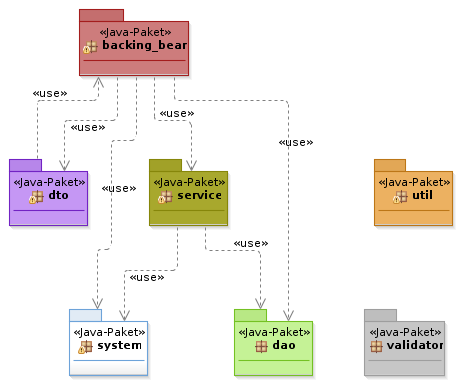
\includegraphics[scale=0.6]{Paketdigram.png}
        \caption{Paketdiagramm}
        \label{fig:Paketdiagramm}
    \end{figure}




%--JSF-Dialoge-----------------------------------------------------------------------------------------------------------------------------------------------------------------------
\section{JSF-Facelets}
\sectionauthor{León Liehr}

\newcommand{\PUB}{jeder}
\newcommand{\USR}{ang. Nutz.}
\newcommand{\ANO}{abg. Nutz.}
\newcommand{\BIB}{Bib.-Mit.}
\newcommand{\ADM}{Admin.}

Nachfolgend verwenden wir die diese Abkürzungen:

\begin{table}[H]
\begin{tabular}{rl}
\toprule
%\PUB & jeder \\
\ANO & abgemeldeter Nutzer \\
\USR & angemeldeter Nutzer \\
\BIB & Bibliotheksmitarbeiter \\
\ADM & Administrator \\
\bottomrule
\end{tabular}
\end{table}

\newcommand{\facelet}[2]{\subsection{#1 (\texttt{#2.xhtml})}}

\newcommand{\BTN}{Knopf}
\newcommand{\LNK}{Hyperlink}
\newcommand{\INP}{Eingabefeld}
\newcommand{\DRP}{Drop-Down-Liste}
\newcommand{\TBL}{Tabelle}

\newenvironment{controls}
{
\begin{table}[H]
\begin{minipage}{\textwidth}
\renewcommand{\thefootnote}{\thempfootnote}
\begin{tabular}{llr}
\toprule
\textbf{Typ} & \textbf{Beschreibung} & \textbf{Sichtbarkeit}\\
\midrule
}{
\bottomrule
\end{tabular}
\end{minipage}
\end{table}
}

\facelet{Seitenvorlage}{template}

\begin{controls}
\BTN\footnote{Dargestellt als Fragezeichenbildsymbol} & zum Anzeigen der kontextsensitiven Hilfe & \PUB\\
\LNK & zu der erweiterten Suche & \PUB\\
\INP & für die Mediensuche & \PUB\\
\LNK & zur Datenschutzerklärung & \PUB\\
\LNK & zum Impressum & \PUB\\
\LNK & zum Kontakt & \PUB\\
\LNK & zu der Profilseite & \USR\\
\LNK & zum Abmelden; zur Anmeldemaske & \USR\\
\LNK & zur Anmeldemaske & \ANO\\
\LNK & zur Registrierungsseite  & \ANO\\
\LNK & zu den abzuholenden Exemplaren & \BIB\\
\LNK & zu der Medienrückgabe & \BIB\\
\LNK & zu der Direktausleihe & \BIB\\
\LNK & zu der Verwaltung & \ADM\\
\end{controls}

\facelet{Abzuholende Exemplare}{copies-ready-for-pickup}

\begin{controls}
\TBL & aller abzuholenden Exemplare & \BIB\\
\BTN & nächste Seite der obigen Tabelle & \BIB\\
\BTN & vorige Seite der obigen Tabelle & \BIB\\
\end{controls}

\facelet{Abzuholende und ausgeliehene Exemplare}{my-copies}

\begin{controls}
\TBL & aller abzuholenden Exemplare & \USR\\
\BTN & nächste Seite der obigen Tabelle & \USR\\
\BTN & vorige Seite der obigen Tabelle & \USR\\
\TBL & aller ausgeliehenen Exemplare & \USR\\
\BTN & nächste Seite der obigen Tabelle & \USR\\
\BTN & vorige Seite der obigen Tabelle & \USR\\
\end{controls}

\facelet{Anmeldemaske}{login}

\begin{controls}
\INP & für die E-Mail-Adresse & \PUB\\
Passworteingabefeld & & \PUB\\
\BTN & zum Anmelden & \PUB\\
\BTN\footnote{Dargestellt als \LNK, um unauffälliger zu sein, da es eine zweitrangige Aktion ist} & zum Passwortzurücksetzen & \PUB\\
\end{controls}

\facelet{Datenschutzerklärung}{privacy-policy}

\begin{controls}
\INP & für die Datenschutzerklärung & \ADM\\
\BTN & zum Speichern der Änderungen an der D. & \ADM\\
\end{controls}

\facelet{Direktausleihe}{direct-lending}

\begin{controls}
\INP & für die E-Mail-Adresse des Ausleihendens & \BIB\\
\INP\footnote{Beim Laden der Seite fünfmal vorhanden. Durch das Pressen des relevanten Knopfs wird ein weiteres Feld angehängt} & für die Signatur eines auszuleihenden Exemplars  & \BIB\\
\BTN & zum Hinzufügen eines weiteren Signaturfelds & \BIB\\
\BTN & zum Ausleihen & \BIB\\
\end{controls}

\facelet{E-Mail-Bestätigung}{email-confirmation}

\facelet{Fehlerseite}{error}

\facelet{Impressum}{site-notice}

\begin{controls}
    \INP & für das Impressum & \ADM\\
    \BTN & zum Speichern der Änderungen am Impressum & \ADM\\
\end{controls}

\facelet{Kategorienbearbeitung}{category-editor}

\begin{controls}
\INP & für den Kategorienamen & \BIB\\
\INP & für die Kategoriebeschreibung & \BIB\\
\BTN & zum Speichern der Änderungen & \BIB\\
\end{controls}

\facelet{Kategorierenstöberer}{category-browser}

\begin{controls}
\INP & für den Suchterm der Kategoriensuche & \PUB\\
\LNK & zur Kategorienbearbeitung (hier: Erstellung) & \BIB\\
\BTN & zum Löschen einer Kategorie & \BIB\\
\LNK & zur Medienerstellung\footnote{unter der aktuellen Kategorie} & \BIB\\
\end{controls}

\facelet{Kontakt}{contact}

\facelet{Leihfristverstöße}{lending-period-violations}

\begin{controls}
\TBL & von Exemplaren und Nutzern & \ADM\\
\BTN & nächste Seite der obigen Tabelle & \ADM\\
\BTN & vorige Seite der obigen Tabelle & \ADM\\
\end{controls}

\facelet{Medienerstellung}{media-creation}

\begin{controls}

\end{controls}

\facelet{Medienrückgabe}{return}

\begin{controls}

\end{controls}

\facelet{Mediensuche}{media-search}

\begin{controls}
\INP & für den Suchterm der freien Suche & \PUB\\
\BTN & zur Durchführung der Suche & \PUB\\
\DRP\footnote{
Beim Laden der Seite dreimal vorhanden, jeweils einmal pro Dreiergruppe bestehend aus mit \footnotemark[\value{mpfootnote}] markierten Elementen.
Durch das Pressen des relevanten Knopfs wird eine weitere Dreiergruppe angehängt
} & für den Suchoperator & \PUB\\
\DRP\footnotemark[\value{mpfootnote}] & für das Suchkriterium & \PUB\\
\INP\footnotemark[\value{mpfootnote}] & für den Suchterm der diff. Suche & \PUB\\
\BTN & zum Hinzufügen eines weiteren Suchfelds & \PUB\\
\TBL & aller Suchergebnisse (falls vorhanden) & \PUB\\
\BTN & nächste Seite der obigen Tabelle & \PUB\\
\BTN & vorige Seite der obigen Tabelle & \PUB\\
\end{controls}

\facelet{Mediumsansicht}{medium}

\begin{controls}
\LNK & zurück zur Trefferliste (Mediensuche) & \PUB\footnote{Nur sichtbar, falls der Nutzer von der Suche kommt}\\
\INP\footnote{Existiert pro Medienattribut} & für ein Medienattribut & \BIB\\
\BTN & zum Speichern der Änderungen an den Medienattributen & \BIB\\
\BTN & zur Bindung an die Abholung des Mediums & \USR\footnote{Nur, falls dem Nutzer erlaubt ist auszuleihen}\\
Zeitdauereingabefeld & für die Rückgabefrist & \BIB\\
\BTN & zum Speichern der Änderungen an der Rückgabefrist & \BIB\\
\LNK & zum Löschen des Mediums; zur zuvor aufgerufenen Seite & \BIB\\
\TBL & aller Exemplare & \PUB\\
\BTN\footnote{existiert pro Exemplar in der Tabelle} & zum Löschen eines Exemplars & \BIB\\
\BTN\footnotemark[\value{footnote}] & zum Stornieren einer Abholung & \BIB\\
\LNK\footnotemark[\value{footnote}] & zur Direktausleihe & \BIB\\
% @Task add footnote at \USR (a previous one)
\BTN\footnotemark[\value{footnote}] & zur Bindung an die Abholung des Mediums & \USR\\
\INP & für den Standort eines neuen Exemplars & \BIB\\
\INP & für die Signatur eines neuen Exemplars & \BIB\\
\BTN & zum Erstellen eines Exemplars & \BIB\\
\end{controls}

\facelet{Mediumschemabearbeitung}{medium-schema-editor}

\begin{controls}

\end{controls}

\facelet{Nutzersuche}{user-search}

\begin{controls}
    \INP & für den Suchterm & \ADM\\
    \BTN & zur Durchführung der Suche & \ADM\\
    \TBL & aller Suchergebnisse (falls vorhanden) & \ADM\\
    \BTN & nächste Seite der obigen Tabelle & \ADM\\
    \BTN & vorige Seite der obigen Tabelle & \ADM\\
\end{controls}

\facelet{Passwortzurücksetzung}{password-reset}

\begin{controls}
Passworteingabefeld & für das neue Passwort & \PUB\\
Passworteingabefeld & zur Bestätigung & \PUB\\
\BTN & zum Zurücksetzen des Passworts & \PUB\\
\end{controls}

\facelet{Profilseite}{profile}

\begin{controls}
\INP & für den Vornamen & \USR\\
\INP & für den Nachnamen & \USR\\
Passworteingabefeld & & \USR\\
Passworteingabefeld & zur Bestätigung & \USR\\
\INP & für die E-Mail-Adresse & \USR\\
\INP\footnote{bzw. getrennt in Ort, PLZ, Straße, Hausnummer} & für die Adresse & \USR\\
\DRP & für die Nutzerrolle & \ADM\\
Checkbox & für den Accountstatus (gesperrt / entsperrt) & \ADM\\
Checkbox & für den Ausleihstatus (gesperrt / entsperrt) & \ADM\\
\INP & für die Rückgabefrist & \ADM\\
\BTN & zum Speichern der Änderungen an den Benutzerdaten & \USR\\
\LNK & zu den abzuholenden und ausgeliehenen Exemplaren & \USR\\
\BTN & zum Schließen des Accounts; zur Anmeldemaske & \USR\\
\BTN & zum Löschen des Nutzers; zur Verwaltungsseite & \ADM\\
\end{controls}

\facelet{Registrierungsseite}{registration}

\begin{controls}
\INP & für den Vornamen & \USR\\
\INP & für den Nachnamen & \USR\\
Passworteingabefeld & & \USR\\
Passworteingabefeld & zur Bestätigung & \USR\\
\INP & für die E-Mail-Adresse & \USR\\
\INP\footnote{bzw. getrennt in Ort, PLZ, Straße, Hausnummer} & für die Adresse & \USR\\
\DRP & für die Nutzerrolle & \ADM\\
\BTN & zum Registrieren des Accounts & \ANO/\ADM\\
\end{controls}

\facelet{Verwaltungsseite}{administration}

\begin{controls}
\INP & für die Rückgabefrist & \ADM\\
\INP & für den Mahnungszeitpunkt & \ADM\\
\INP & für die Abholfrist & \ADM\\
\INP & für den Systemnamen & \ADM\\
Checkbox & für den Zugangsstatus (anonym oder nicht) & \ADM\\
Checkbox & für den Registrierungsstatus & \ADM\\
\INP & für den regulären Ausdruck valider E-Mail-Adressen & \ADM\\
Farbkreis\footnote{Alternativ ein einfaches \INP} & für die erste Farbe des Systems & \ADM\\
Farbkreis\footnotemark[\value{footnote}] & für die zweite Farbe des Systems & \ADM\\
Datei-Upload & für das Logo des Systems & \ADM\\
\BTN & zum Speichern der Änderungen an den Systemeinstellungen & \ADM\\
\LNK & zu der Medienerstellung & \ADM\\
\LNK & zu der Registrierungsseite (fremden Nutzer erstellen) & \ADM\\
\LNK & zur Mediumsschemabearbeitung & \ADM\\
\LNK & zu den Leihfristverstößen & \ADM\\
\LNK & zu der Nutzersuche & \ADM\\
\INP & für den Suchterm der Nutzersuche & \ADM\\
\end{controls}

%--Systemfunktionen----------------------------------------------------------------------------------------------------------------------------------------------------------------
\section{Systemfunktionen}
\sectionauthor{Jonas Picker}
\subsection{Technische Systemsicherheit}
\noindent \textbf{Kommunikationsverschlüsselung:} Durch das vorrausgesetzte SSL-Zertifikat des Tomcat-Servers wird der Anwendung die Kommunikation mit dem HTTPS-Protokoll ermöglicht. Dies ist eine Ergänzung der HTTP-Kommunikation um eine Transportverschlüsselung. Zusätzlich zur Vereitelung von Abhörversuchen der an Ihren Server gesendeten Anfragen signalisieren Sie den Klienten so auch die Vertrauenswürdigkeit Ihrer Institution durch die CA\footnote{'Certification Authority' - eine digitale Zertifizierungsstelle}-Zertifizierung.\\
\textbf{Nutzerberechtigungen:} Um zu Verhindern, dass Nutzer ohne ausreichende Berechtigungen auf zugangsbeschränkte Bereiche des Webspaces zugreifen können, werden entsprechende Maßnahmen ergriffen: Um den direkten Aufruf von Seiten, die für den Nutzer nicht zugänglich sein sollten, zu unterbinden, verwenden wir einen sogenannten Phaselistener. Wie jede JSF-Anwendung durchläuft auch unsere nach Erhalt einer Anfrage eine Reihe von Verarbeitungsphasen, bevor die Antwort an den Klienten fertiggestellt und verschickt wird. Ein Phaselistener kann während dieses Prozesses zusätzliche Integritätsbedingungen abprüfen und gegebenenfalls die Antwort auf die Anfrage verändern/verhindern. Zusätzlich wird durch das in JSF eingebaute Session-Tracking\footnote{Das Verfolgen der Klientenverbindung zwischen den eigentlich verbindungslosen HTTP-Anfragen} sichergestellt, dass die verschiedenen Nutzerrollen eine unterschiedliche Version der gleichen Seiten angezeigt bekommen, deren Funktionalitäten den Berechtigungen der Rollen entsprechen. Es wird durch das manuelle Austauschen des Identifikators für die Nutzer-Session an kritischen Stellen dafür gesorgt, dass Nutzer vor Session-Hijacking\footnote{Das Stehlen einer validen Nutzer-Session um Zugriff auf den Account und seine Berechtigungen zu erhalten} geschützt werden.\\
\textbf{Vorbeugen von Angriffen:} Durch geschicktes Einschleusen von SQL\footnote{'Structured Query Language' - eine weit verbreitete Datenbankanfragesprache}-Code in ungesicherte Formularfelder könnten Unbefugte direkten Zugriff auf die darunterliegende Datenbank erhalten. Der Datenbankzugriff in unserem System erfolgt via JDBC\footnote{'Java Database Connectivity' - eine universelle Datenbankschnittstelle}, welche bereits über einen Mechanismus zur Verhinderung von diesen SQL-Injections verfügt. Hierbei wird verhindert, dass von Nutzern eingegebener Text vom Managementsystem der Datenbank interpretiert wird. Ein weiterer Angriffsvektor stellt das sogenannte Cross-Site-Scripting dar. Dabei wird versucht, nutzergenerierte Teile von Websiten mit vom Browser interpretierbaren Codeabschnitten zu füllen, welche dann beim Anzeigen des Inhalts bei anderen Klienten ausgeführt werden. Es gibt verschiedene Versionen dieser Angriffsart, von denen nicht alle am Server verhindert werden können. Jedoch wird in der Anwendungslogik jede Nutzereingabe auf interpretierbaren HTML (und eingebundenen JavaScript) Code untersucht und gegebenenfalls entschärft.
\subsection{Fehlerbehandlung und Logging}
Von uns vorhergesehene Fehler und einige im Hintergrund ablaufende Prozesse werden durch einen selbst erstellten Logging-Mechanismus dokumentiert. Da dieser Mechanismus während des Entwicklungsprozesses ebenfalls nützlich ist und auf feinster Einstellung für den Anwender uninteressant sein könnte, wird es eine Option geben, die den Detailgrad und die Anzahl der ausgegebenen Meldungen festlegt. Alle Meldungen werden in eine seperate Log-Datei geschrieben und können wahlweise auf der Konsole angezeigt werden. Vorhergesehene Fehler in Abläufen werden von der Anwendung bestmöglich abgehandelt und wie erwähnt durch das Logging dokumentiert/kommuniziert. Sollte jedoch ein nicht vorhergesehener Fehler auftreten, wird der Grund dafür in Form der Java-eigenen Exceptions auf die Konsole ausgegeben. Durch umfangreiches Testen der Anwendung vor Auslieferung versuchen wir, solche Fehlerquellen zu finden und zu beheben. Im Optimalfall kommen Sie nicht mit unvorhergesehen Fehlern in Berührung. Sollten sie dennoch auftreten, wenden Sie sich bitte direkt an uns.
\subsection{Selbstständige Prozesse}
Im System gibt es verschiedene Fristen (Abholungsmarkierung, Ausleihrückgabe [global, pro Medium, pro Nutzer], Gültigkeit des Verifizierungs-/Zurücksetzungslinks, Mahnungszeitversatz) und damit verbundene Aktionen. Um diese Aktionen ausführen zu können, muss das System in gewissen Abständen selbstständig auf die Datenbank zugreifen. In der Klasse ???? ist dafür ein eigener Wartungsthread implementiert.
\subsection{Starten und Stoppen der Anwendung}
\noindent \textbf{Start:} Beim Systemstart wird zunächst der oben beschriebene Logging-Mechanismus initialisiert. Im Anschluss liest das System die Konfigurationsdatei ein und versucht die dort angegebene Verbindung zur Datenbank. Bei erfolgreicher Verbindung wird überprüft, ob die benötigten Tabellennamen alle existieren bzw. legt diese bei deren Fehlen an. Sollte die Struktur der Tabellen fehlerhaft sein, wird eine Fehlermeldung geloggt und die Tabellen werden nicht vom System benutzt. Wenn die Datenbank fehlerhaft/nicht verbunden ist, werden eingehende Anfragen mit einer Fehlerseite beantwortet. Nach erfolgreichem Ablauf der vorhin genannten Prozesse wird als nächstes der Wartungsthread angestoßen, um fristenabhängige Aktionen durchzuführen. Danach ist das System vollständig betriebsbereit.\\
\textbf{Stop:}
Beim planmäßigen Herunterfahren des Systems werden zunächst die noch offenen Datenbankverbindungen geschlossen und danach die Anwendung gestoppt. Da dies sehr schnell passiert, wird währenddessen auf eine extra Umleitung der Nutzer auf eine Fehlerseite verzichtet. Da unsere SQL-Transaktionen dem ACID\footnote{'Atomicity, Consistency, Isolation, Durability' - ein Leitsatz von Eigenschaften für Datenbanktransaktionen}-Prinzip folgen, wird die Datenbank jedoch auch beim Herunterfahren während eines Zugriffs in konsistentem Zustand hinterlassen. Nutzersessions überleben das Ausschalten des Servers nicht, d.h. alle eingeloggten Nutzer sind nach einem Neustart des Systems ausgeloggt. Wenn die Java Laufzeitumgebung des Systems plötzlich beendet wird und das System abstürzt, wird mittels einer sogenannten ShutdownHook trotzdem noch versucht, offene Datenbankverbindungen zu schließen. Dies ist bei einem Stromausfall allerdings unmöglich.
%--Datenfluss--------------------------------------------------------------------------------------------------------------------------------------------------------------------------
\section{Datenfluss}
\sectionauthor{Sergei Pravdin}
Die Kommunikationen zwischen den Klassen und die Interaktionen des Systems werden durch den Sequenzdiagramme abgebildet. Um einen Datenfluss beispielhaft zu zeigen, werden die zwei Szenarien vorgelegt. Zuerst bucht ein angemeldeter Nutzer ein Medium-Exemplar erfolgreich zur Ausleihe. Im zweiten Szenario bucht ein angemeldeter Nutzer ein Medium-Exemplar erfolglos zur Ausleihe, weil die Verbindung mit der Datenbank fehlgeschlagen ist.
\subsection{Interaktionen beim erfolgreichen Buchen eines Medium-Exemplars}
Der Nutzer befindet sich auf der Mediensuche-Seite und wünscht das Buch 'Programmieren lernen' zu buchen. Im System existiert das Medium mit dem Titel 'Programmieren lernen' und der Signatur '17RE'. Ein Exemplar mit der Signatur '17RE (+1)' gehört zu dem genannten Medium. Das System ist so eingestellt, dass die angemeldeten Nutzer Zugriff auf den Medien haben.
\subsubsection{Suchen nach dem Medium}
Der Nutzer gibt 'Programmieren lernen' und '17RE' in die Suchfelder 'Titel' und 'Signatur' und klickt auf den Suchen-Button. Das Mediensuche-Bean kapselt die Sucheingabe ins Mediensuche-DTO ein. Das Mediensuche-DTO ruft die Methode 'getMedien' aus dem Mediensuche-DAO auf. Das Mediensuche-DAO ruft die Methode 'getConnection' aus dem Connection-Pool-Bean und bekommt eine Connection von dem zurück. Danach führt das Mediensuche-DAO eine selectSQL-Anfrage durch und gibt eine Liste der entsprechenden Medien dem Mediensuche-DTO zurück. Im nächsten Schritt leitet Mediensuche-DTO diese Liste der Medien dem Mediensuche-Bean weiter. Das Mediensuche-Bean ruft seine Methode 'updateMedien' auf und gibt dem Nutzer die aktualisierte Mediensuche-Seite zurück.
\subsubsection{Navigation zum Medium}
Der Nutzer klickt auf das angezeigte Medium 'Programmieren lernen'. Das Mediensuche-Bean ruft die Methode 'navigate' auf und gibt die Mediumsansicht-Seite zurück.
\subsubsection{Buchen eines Exemplares}
Der Nutzer klickt auf den Buchen-Button. Das Medium-Bean ruft die Methode checkStatus aus dem UserSession-Bean auf, um zu prüfen, ob der Nutzer Zugriff zum Buchen hat. Das UserSession-Bean gibt das positive Ergebnis dem Medium-Bean zurück. Das Medium-Bean kapselt das Buchen ins Medium-DTO ein und das Medium-DTO ruft die Methode book() aus dem Medium-DAO auf. Das Medium-DAO ruft die Methode 'getConnection' aus dem Connection-Pool-Bean und bekommt eine Connection von dem zurück. Danach führt das Medium-DAO eine updateSQL-Anfrage durch. Im nächsten Schritt gibt Medium-DTO  dem Medium-Bean das Ergebnis der Operation zurück. Das Medium-Bean ruft seine Methode 'updateExamples' auf und gibt dem Nutzer die aktualisierte Medium-Seite zurück. Das Exemplar ist erfolgreich gebucht.

\newpage
\newgeometry{left=0cm,right=0cm,top=0.5cm,bottom=0cm}

\begin{figure}[h]
    \centering
    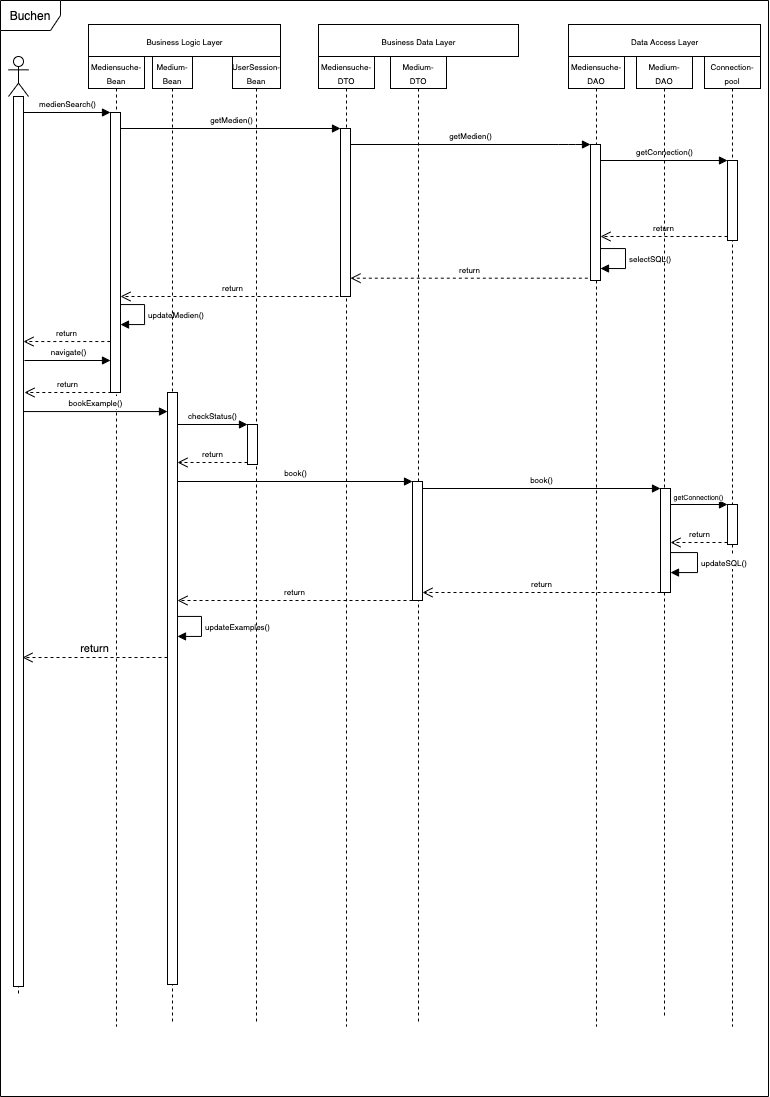
\includegraphics[width = 45em]{Sequenzdiagramm-2}
    \caption{Interaktionen bei einem erfolgreichen Buchen eines Medium-Exemplars}
    \label{Sequenzdiagramm}
\end{figure}

\restoregeometry
\newpage

%--ER-Modell--------------------------------------------------------------------------------------------------------------------------------------------------------------------------
\section{ER-Modell}
\sectionauthor{Jonas Picker}

\newpage
\newgeometry{left=0cm,right=0cm,top=0cm,bottom=0cm}

\begin{figure}[h]
    \centering
    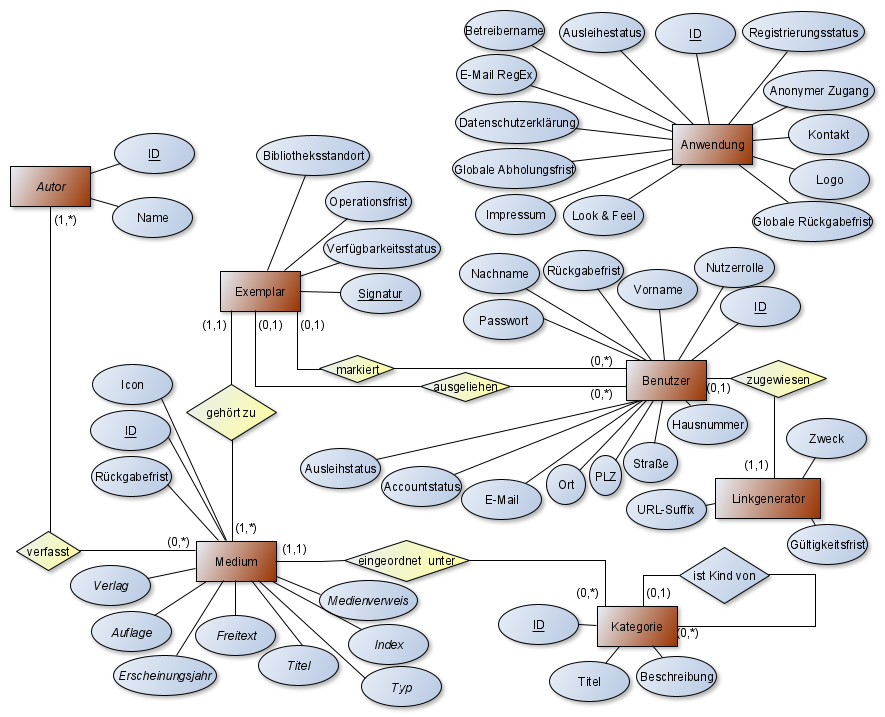
\includegraphics[angle = 270, width = 60em]{ER-Diagramm}
    \caption{Entity-Relationship Diagramm}
    \label{ER-Diagramm}
\end{figure}

\restoregeometry
\newpage

\subsection{Legende}
Jede Entität wird im Folgenden zusammen mit ihren nicht offensichtlichen Attributen und Relationen kurz beschrieben.\\
\textbf{Medium:} Diese Entität modelliert die in der Bibliothek gehaltenen Medien. Zusätzlich zum Primär-schlüssel ist auch das Attribut 'Rückgabefrist' und 'Icon' nicht vom Administrator entfernbar, die restlichen Attribute (kursiv) stellen den modifizierbaren Standartsatz der Medienattribute dar (PfHft. /D020/). Erwähnenswert ist hier noch das als mehrwertig markierte, editierbare Attribut 'Autoren', diese Markierung kann auch zu benutzerdefinierten Attributen hinzugefügt werden und wird mit dem Anlegen einer neuen Entität modelliert (PfHft. /F380/).\\
\textbf{Kategorie:} Die mit dieser Entität verbundenen Relationen ordnen jedem Medium genau eine Kategorie zu und modellieren die Kategoriehierarchie (PfHft. /W440/) durch die Selbstbeziehung. Es wird einen unlöschbaren Top-Knoten in der Hierarchie geben, zu dem alle Medien, die nie in eine Kategorie eingeteilt wurden oder deren Kategorie gelöscht wurde, gehören. Sollten alle Medien in benutzerdefinierten Kategorien stecken, hat der Top-Knoten keine zugeordneten Medien und nimmt somit nicht an der 'eingeordnet unter'-Relation teil.\\
\textbf{Exemplar:} Von jedem Medium muss mindestens ein Exemplar vorhanden sein. Auch kann ein bestimmtes Exemplar von genau einem Nutzer zur Abholung markiert oder ausgeliehen werden, diese Aktionen schließen sich gegenseitig aus (PfHft. /F310/) und ändern (genau wie eine Rückgabe) den Verfügbarkeitsstatus und die dazugehörige Operationsfrist dementsprechend. \\
\textbf{Benutzer:} Ob ein Benutzer die Ausleihfunktion benutzen kann, wird durch das Attribut 'Ausleihstatus' modelliert. 'Accountstatus' zeigt hingegen an, ob der Nutzeraccount bereits den Verifizierungsprozess durchlaufen hat (PfHft. /W70/). Das Passwort wird in gehashter Form abgespeichert. \\
\textbf{Linkgenerator:} Diese Entität kapselt einen befristet gültigen URL-Suffix, aus dem der Verifizierungs- oder Passwortzurücksetzungslink (je nach Zweck) für genau einen Account erstellt wird.\\
\textbf{Anwendung:} Hier werden die setzbaren globalen Variablen und Anwendungseinstellungen gespeichert. Diese Tabelle hat nur einen einzigen Eintrag. 'Anonymer Zugang' modelliert die Berechtigungen anonymer Nutzer beim Besuchen des Webspaces (PfHft. /F10/), während 'Registrierungsstatus' eine nutzerfreundlichere Alternative als den RegEx zum Sperren der Registrierung bietet (PfHft. /F20/). 'Ausleihstatus' steht für das Umschalten des Systems zur manuellen Freischaltung der Ausleihfunktion für registrierter Nutzer. 'Look \& Feel' speichert das momentan ausgewählte Farbschema. \\

\end{document}

